\section{Method}
\label{sec:method}

\subsection{Teacher: which world model and why}
The teacher is \vjepa ViT-B~\cite{assran2025vjepa2,vjepa21_2026}, a self-supervised video model trained by predicting
masked latent features rather than pixels. Three properties make it the right teacher for a wiring question. Its
latent is \emph{action-free and generic}, so nothing about navigation is baked into the target. It is \emph{causal
per step} in our use: each environment step is duplicated into a 16-frame tubelet that ends at $t$, so a blind
target never contains frames the student has not seen. And it is \emph{cheap to regress}: the mean token concatenated
with $2\times2$ pooled tokens (3,840-d) is projected to a PCA-256 basis fit on the training set (94.6\,\% variance on the
arena, 91.0\,\% on NYC) and whitened by one scalar. All MSE values are in this whitened space. The teacher's weights
are never touched; it is a target generator.

\subsection{Distillation: which technique and why}
We use response-based latent regression, the plainest member of the distillation
family~\cite{hinton2015distilling}: the student's linear readout must match the teacher's latent at every step,
\begin{equation}
  \mathcal{L} = \sum_t w_t\,\big\lVert W_{\rm out} h_t - z_t\big\rVert^2 + 10^{-4}\,\overline{h^2},
  \label{eq:loss}
\end{equation}
with $w_t=3$ on blind steps and $1$ otherwise,
and no feature-alignment, no logit or attention matching and no policy term. The blind steps are the point: during a
random contiguous window the visual input is zeroed and only the action is given, so the student must carry the
teacher's latent forward from the action record. Feature-level distillation~\cite{romero2015fitnets} was rejected
because the student has no layers to align; transformer-to-RNN hidden-state matching~\cite{bick2024transformers} was
rejected because the student's state is a set of named neurons, not a free vector. Anything the state learns about
heading or position is therefore a by-product of \cref{eq:loss}.

\subsection{Connectome subgraph}
\label{sec:connectome}
From \flywire v783~\cite{dorkenwald2024neuronal,schlegel2024whole} we take 6,935 neurons in four populations
(\cref{fig:pipeline}): VIS (2,330; TuBu, MeTu, LC and LPLC visual projection neurons), CX (2,875; every central-complex
class, including EPG, PEN, $\Delta$7, PFN, PFL, h$\Delta$, FC, ER and ExR), MB (427; mushroom-body output and
dopaminergic neurons) and OUT (1,303; descending neurons). Edges are the 91,663 directed pairs with at least 5
synapses; 40,194 of them cross the midline. Each edge's sign is the predicted neurotransmitter of its presynaptic
neuron~\cite{eckstein2024neurotransmitter} (ACh, DA, 5-HT, OA excitatory; Glu, GABA inhibitory; 49.9\,\% excitatory),
so Dale's law holds by construction. The optic lobe (about 70k neurons) is omitted because it would dominate the
neuron count while adding nothing the teacher latent does not already encode. \Cref{sec:ablation} ablates the synapse
threshold and the region choice.

\subsection{Student}
\label{sec:student}
\begin{figure}[t]
  \centering
  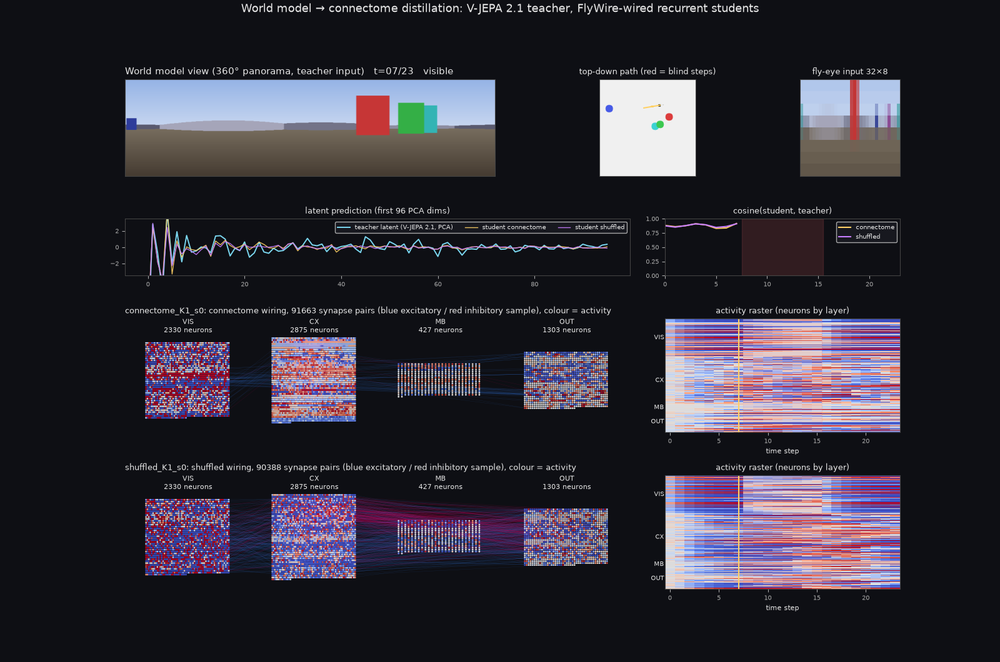
\includegraphics[width=0.49\linewidth]{fig/wm2cx_connectome_t07.png}\hfill
  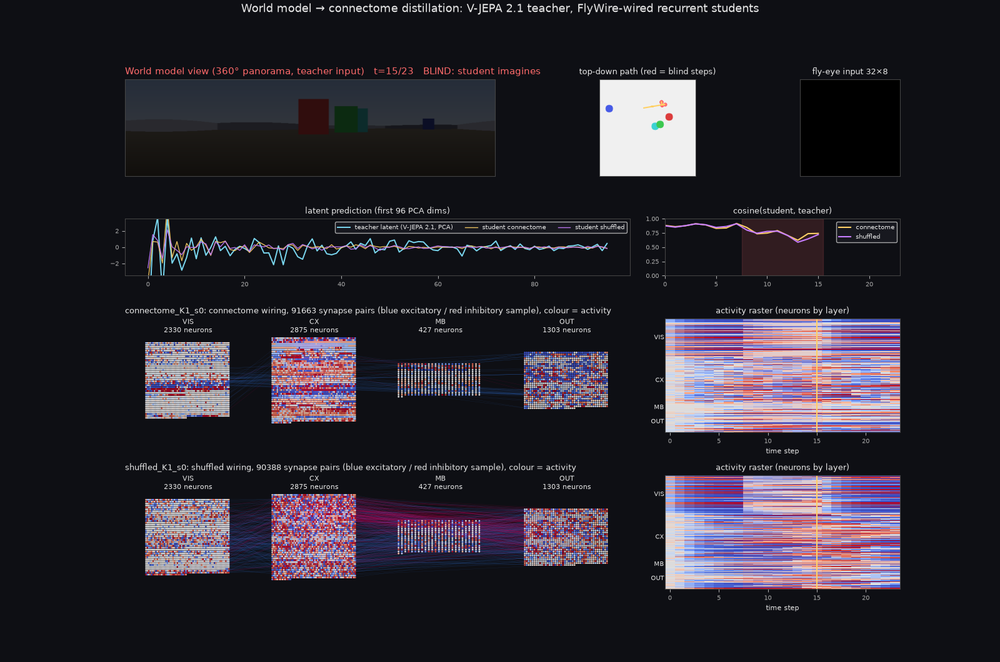
\includegraphics[width=0.49\linewidth]{fig/wm2cx_connectome_t15.png}
  \caption{\textbf{The student's state is a set of named neurons.} Activity of all 6,935 neurons at their \flywire soma
  positions, eyes open (left, step 8) and eyes closed (right, step 16) in the arena. Because every unit is a real cell
  with a cell type and a hemisphere, probes can be asked of populations (EPG, CX, VIS) and not only of the whole state.}
  \label{fig:activity}
\end{figure}
The student is a leaky tanh rate network on the connectome's neurons,
\begin{equation}
  h_{t+1} = (1-\alpha)\,h_t + \alpha\tanh\!\big(g\,(W h_t + W_{\rm in}\, o_t v_t + W_{\rm act}\, a_t + b)\big),
  \label{eq:student}
\end{equation}
with $\alpha=0.5$, gain $g$, fly-eye input $o_t$ ($32\times8\times3$) gated by the visibility flag $v_t$ and one-hot
action $a_t$. $W$ is non-zero only on connectome edges and parametrised as $W_{ij}=s_{ij}\,\mathrm{softplus}(w_{ij})$
with $s_{ij}$ fixed, so training can change synaptic strength but never sign or existence. Visual input enters VIS
neurons only; the action enters CX and OUT; the readout is linear from all neurons. The recurrence has 91,663
parameters; $W_{\rm in}$ and the readout add 3.6\,M, identical for every sparse wiring. One step costs $O(E)$.

\subsection{Single connectome versus multiple connectomes}
\label{sec:multi-method}
\begin{figure}[t]
  \centering
  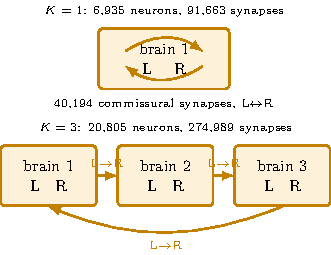
\includegraphics[width=\linewidth]{fig/multi.pdf}  % source: fig/src/multi.tex (build: fig/src/build.sh)
  \caption{\textbf{One brain or several.} For $K>1$ the whole subgraph is cloned $K$ times. Ipsilateral synapses stay
  inside each copy; each of the 40,194 contralateral synapses is moved so that it connects copy $k$ to copy $k+1$
  (modulo $K$). No new edge is invented, so the multi-brain student is still a real wiring diagram, and the input
  and readout maps are shared, so the parameter count grows only by the synapses.}
  \label{fig:multi}
\end{figure}
A single fly brain has a fixed neuron count. To ask whether the connectome is \emph{capacity}-limited rather than
\emph{wiring}-limited we clone the whole subgraph $K$ times and couple the copies through the real commissural
edges only (\cref{fig:multi}). The construction keeps every control valid: edge count scales exactly by $K$, degrees
are preserved per copy, and Dale's signs are untouched. We run $K\in\{1,2,3\}$ with five seeds each.

\subsection{Sparse state versus dense state: the controls}
\label{sec:controls}
\begin{figure}[t]
  \centering
    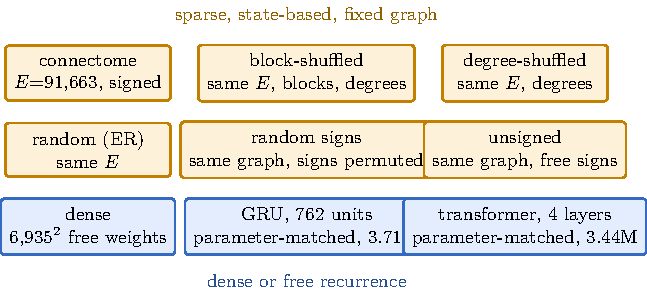
\includegraphics[width=\linewidth]{fig/controls.pdf}  % source: fig/src/controls.tex (build: fig/src/build.sh)
  \caption{\textbf{Nine recurrent cores at one input, one readout, one loss.} Orange (top two rows) cores share the neuron set,
  region labels, I/O routing, edge count and Dale-consistent sign fraction and differ only in which synapses exist or
  which neurons are excitatory. Blue (bottom row) cores are what current latent world models use. Block-shuffled is the decisive
  control: it keeps the macro-architecture and destroys only synapse identity.}
  \label{fig:controls}
\end{figure}
Every sparse control (\cref{fig:controls}) keeps the neuron set, the region labels, input and output routing, the
exact edge count, no self-loops and Dale-consistent signs at the real excitatory fraction. \textbf{Block-shuffled}
applies Maslov--Sneppen rewiring~\cite{maslov2002specificity} inside each region-to-region block, preserving per-block
in- and out-degrees and all block edge counts. \textbf{Degree-shuffled} rewires globally. \textbf{Random} is
Erd\H{o}s--R\'enyi at the same edge count. \textbf{Random signs} permutes which neuron is excitatory; \textbf{unsigned}
frees the signs. \textbf{Dense} frees all $6{,}935^2$ weights (51.7\,M). The \textbf{GRU}~\cite{cho2014learning} has 762
units, matched to the sparse student's \emph{total} parameters (3.71\,M); a second GRU with 174 units matches the
connectome's \emph{recurrent} budget (90,828 weights). The \textbf{transformer} is a causal pre-LN predictor in the
style of IRIS, STORM and DINO-WM~\cite{micheli2023iris,zhang2023storm,zhou2024dinowm}, one token per step, the deepest
model within the budget (4 layers, 3.44\,M); its state for every probe is the last token. Two further ablations test
the input side: a \emph{cross-attention input encoder} (each VIS neuron owns a query over the fly-eye patches, 0.11\,M
instead of 1.83\,M parameters) and a \emph{hybrid} that adds one attention layer over 796 cell-type-pooled tokens to
the connectome recurrence. In a second copy of the arena data every turn is $22.5^\circ(1+\epsilon)$,
$\epsilon\sim\mathcal{N}(0,0.3)$, so heading is no longer a linear function of the action counts.

\subsection{Benchmarks}
\label{sec:envs}
\begin{figure}[t]
  \centering
  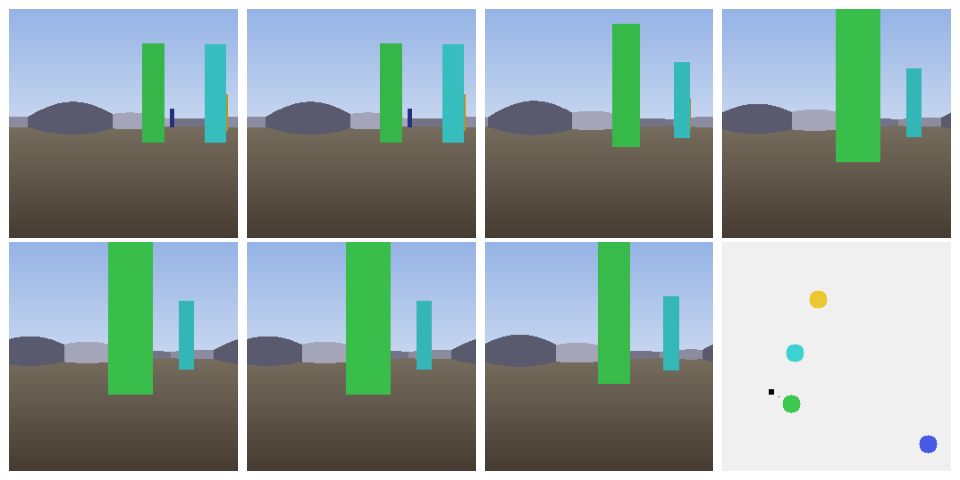
\includegraphics[width=0.49\linewidth]{fig/env_nav.png}\hfill
  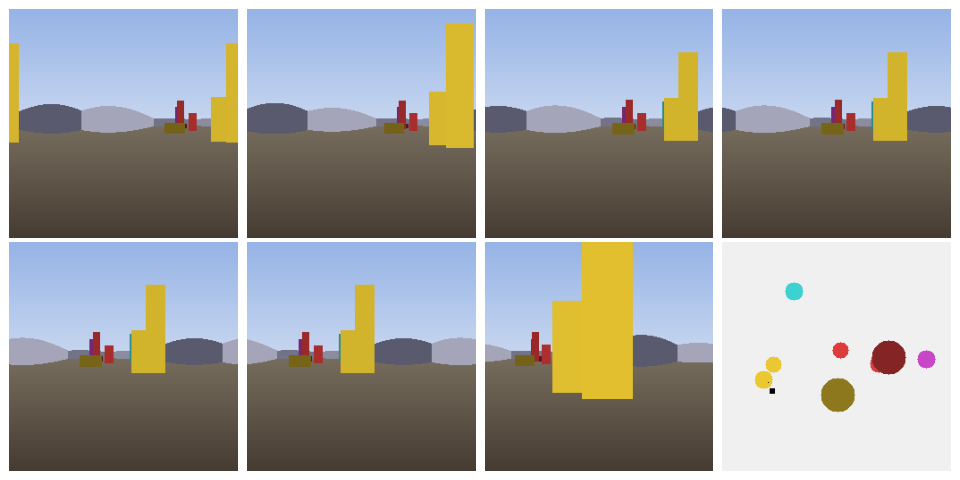
\includegraphics[width=0.49\linewidth]{fig/env_arrange.png}\\[2pt]
  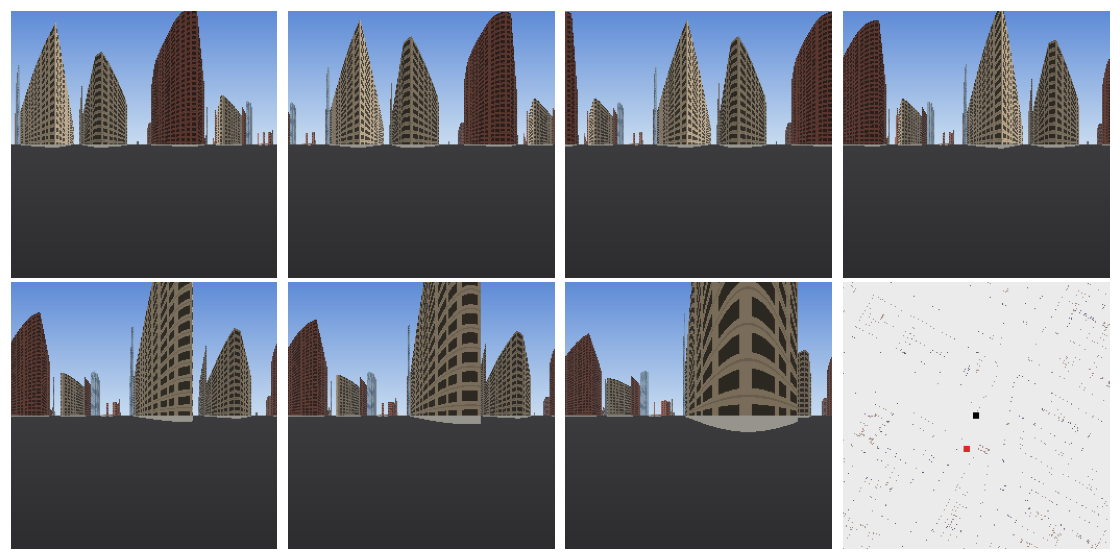
\includegraphics[width=\linewidth]{fig/env_nyc.png}\\[2pt]
  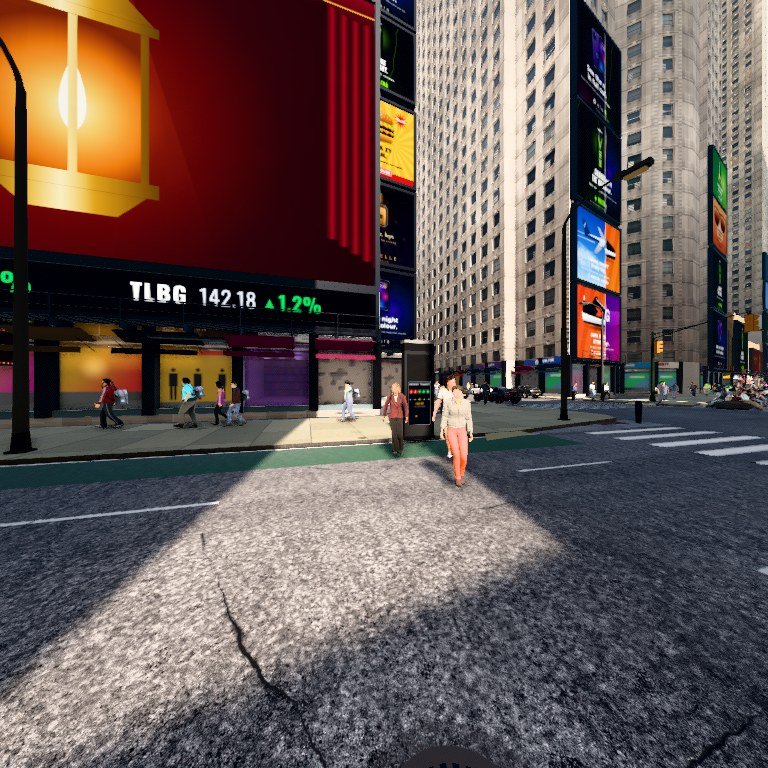
\includegraphics[width=\linewidth]{fig/nyc_hero_0.jpg}
  \caption{\textbf{Three worlds.} Top: the 360\degree\ arena for \textsc{nav} (left) and \textsc{arrange} (right).
  Bottom: seven steps of one episode in the raycast twin of Midtown Manhattan with its top-down map (start black,
  goal red), and the twin rendered at its highest quality (Times Square, ambient traffic and pedestrians). The third world, real phone video, is shown in \cref{fig:realvid}.}
  \label{fig:envs}
\end{figure}
\textbf{Arena.} A 360\degree\ cylindrical panorama at 256\,px with coloured blocks; tasks \textsc{nav} and
\textsc{arrange}; five actions (stay, forward 0.6, turn $\pm22.5$\degree, back 0.36); 24-step scripted episodes; 1,000
train, 200 test. \textbf{NYC twin.} A raycast model of Midtown Manhattan from building footprints; 110\degree\ camera,
forward 4\,m, back 2\,m, goals 30 to 60\,m; 600 episodes split \emph{geographically} into train and test street blocks.
\textbf{Real video.} \nRvClips\ phone clips walked through city streets, \nRvEpisodes\ episodes of 24 steps at 2\,Hz; yaw
and forward motion estimated by patch phase correlation and quantised to the five actions (\cref{sec:suppl-realvid}). A
test set only, except in the leave-one-clip-out fine-tuning condition. \textbf{Blackouts.} Test windows are steps 8 to
16 unless stated (also 8 to 24 and 4 to 24).

\paragraph{Metrics and probes}
Blind latent MSE and cosine in whitened PCA space, mean over horizons 1 to 8, against copy-last and constant-mean
floors. Ridge probes from $h_t$ to heading ($\sin,\cos$) and position relative to the start of the window, fit on
training episodes, reported as median heading error and position $R^2$, against two reference rows: \emph{actions
only} (the same probe on cumulative one-hot actions) and \emph{integrator} (closed-form dead reckoning, the
information ceiling). An MLP probe tests for non-linear codes. \emph{Blind homing}: 12 visible steps, then 24 steps
steered from a pose decoded from the state, success within 1 unit (12\,m on NYC), against oracle pose, dead reckoning
and random actions. \nSeeds\ seeds on the arena, \nSeedsNyc\ on NYC; mean\pm sd and 95\,\% $t$-intervals.
